\documentclass[11pt,a4paper]{jsarticle}

\makeatletter

%%% 個人設定 
\usepackage{amsmath,amssymb}
\usepackage{amsthm}
\usepackage{graphicx}

\bibliographystyle{plain}

\newcommand{\R}{\mathbf R}
\newcommand{\N}{\mathbf N}
\newcommand{\Q}{\mathbf Q}
\newcommand{\Z}{\mathbf Z}
\newcommand{\T}{\{0\}^*}
\newcommand{\D}{D}
\newcommand{\classP}{\mathbf{P}}
\newcommand{\classPSPACE}{\mathbf{PSPACE}}
\newcommand{\classNP}{\mathbf{NP}}
\newcommand{\classPH}{\mathbf{PH}}
\newcommand{\classPP}{\mathbf{PP}}
\newcommand{\classCH}{\mathbf{CH}}
\newcommand{\C}{\mathbf{C}}
\newcommand{\DIVPpoly}{\mathbf{DIVP(\mathrm{poly})}}
\newcommand{\DIVPlog}{\mathbf{DIVP(\log)}}

\theoremstyle{definition}
\newtheorem{theorem}{定理}[section]
\newtheorem{lemma}[theorem]{補題}
\newtheorem{collorary}[theorem]{系}
\newtheorem{definition}[theorem]{定義}
\newtheorem{hypothesis}[theorem]{仮定}

\renewcommand{\proofname}{\bf 証明} 

%%% \proc != 0 ならば証明などをとばす.
\newcommand{\proc}{1}


%%% 数式中の大文字ギリシャ文字を斜体化
\renewcommand{\Lambda}{\varLambda}
\renewcommand{\Gamma}{\varGamma}

%%% (i), (ii), (iii), (iv)
\def\theenumi{\roman{enumi}}
\def\labelenumi{(\theenumi)}

%%% 数式番号を(章.num) に
\renewcommand{\theequation}{\thesection.\arabic{equation}}
\@addtoreset{equation}{section}

%%% 表番号を 章.num に
\renewcommand{\thetable}{\thesection.\arabic{table}}
\@addtoreset{table}{section}

%%% 図番号を 章.num に
\renewcommand{\thefigure}{\thesection.\arabic{figure}}
\@addtoreset{figure}{section}

%%% align* などで指定した場所だけ数式番号を置く
\newcommand{\taghere}{{
\stepcounter{equation}
\tag{\theequation}
}}

\makeatother

\title{滑らかな常微分方程式の計算量}

\author{%
\hspace*{7zw}% 良い子は真似してはいけません!
太田浩行\thanks{東京大学, \texttt{hota@is.s.u-tokyo.ac.jp}} 
\and
河村彰星\thanks{東京大学}%
\hspace*{7zw}% 良い子は真似してはいけません!
\and
マルチン・ツィーグラー\thanks{Martin Ziegler, ダルムシュタット工科大学}
\and
カルステン・レースニク\thanks{Carsten R\"osnick, ダルムシュタット工科大学}
}
%\和暦
\date{}

\begin{document}

\maketitle

%%% 以下に,予稿の本文を記述して下さい.

\begin{abstract}
The computational complexity of the solution~$h$ to 
the ordinary differential equation 
$h(0)=0$, $h'(t) = g(t, h(t))$ 
under various assumptions on the function $g$
has been investigated
in hope of understanding the intrinsic hardness of 
solving the equation numerically. 
Kawamura showed in 2010 that the solution~$h$ can be $\classPSPACE$-hard
even if $g$ is assumed to be Lipschitz continuous and polynomial-time computable. 
We place further requirements on the smoothness of $g$ 
and obtain the following results: 
the solution~$h$ is still $\classPSPACE$-hard
if $g$ is assumed to be of class $\classC ^1$; 
for each $k \geq 2$, 
the solution~$h$ is hard for the counting hierarchy 
if $g$ is assumed to be of class $\classC ^k$. 
\end{abstract}


\section{Introduction}

Let $g \colon [0,1] \times \R \to \R$ be continuous 
and consider the differential equation 
\begin{align}
 \label{eq:ode}
 h(0) & = 0, &
 \D h(t) & = g(t,h(t)) \quad t \in [0,1], 
\end{align}
where $\D h$ denotes the derivative of $h$. 
How complex can the solution~$h$ be, 
assuming that $g$ is polynomial-time computable? 
Here, polynomial-time computability 
and other notions of complexity 
are from the field of 
\emph{Computable Analysis}~\cite{weihrauch00:_comput_analy}
and measure how hard it is to 
approximate real functions with specified precision 
(Section~\ref{section: preliminaries}). 

If we put no assumption on $g$ other than being polynomial-time computable, 
the solution~$h$ (which is not unique in general) can be non-computable. 
Table~\ref{table:related} summarizes known results about 
the complexity of $h$ under various assumptions 
(that get stronger as we go down the table). 
In particular, if $g$ is (globally) Lipschitz continuous, 
then the (unique) solution $h$ is known to be 
polynomial-space computable but still can be 
$\classPSPACE$-hard \cite{kawamura2010lipschitz}. 
In this paper, we study the complexity of $h$ 
when we put stronger assumptions about 
the smoothness of $g$. 

\begin{table}
\renewcommand\arraystretch{1.3}
\begin{center}
 \caption{The complexity of the solution $h$ of \eqref{eq:ode}
 assuming $g$ is polynomial-time computable.}
 \label{table:related}
 \begin{tabular}{lll}
  Assumptions & Upper bounds & Lower bounds \\
  \hline
   --- & --- & can be all non-computable \cite{pour1979computable} \\
  $h$ is the unique solution & computable \cite{coddington1955theory}
  & can take arbitrarily long time \cite{ko1983computational,miller1970recursive} \\
  the Lipschitz condition  & polynomial-space \cite{ko1983computational}
      &	can be $\classPSPACE$-hard \cite{kawamura2010lipschitz}\\
  $g$ is of class $\classC ^{(\infty, 1)}$ & polynomial-space 
      & can be $\classPSPACE$-hard (Theorem~\ref{DifferentiableIsPspace}) \\
  \parbox[t]{11em}{$g$ is of class $\classC ^{(\infty, k)}$\\{}(for each constant $k$)}
  & polynomial-space & can be $\classCH$-hard (Theorem~\ref{KTimesIsCH}) \\
  $g$ is analytic
  & polynomial-time \cite{muller1987uniform,ko1988computing} 
  & ---
 \end{tabular}
\end{center}
\end{table}

In numerical analysis, 
knowledge about smoothness of the input function 
(such as being differentiable enough times) 
is often beneficial 
in applying certain algorithms or simplifying their analysis.
However, 
to our knowledge, 
this casual understanding that smoothness is good 
has not been rigorously substantiated 
in terms of computational complexity theory. 
This motivates us to ask whether, 
for our differential equation \eqref{eq:ode}, 
smoothness really reduces the complexity of the solution. 

At the extreme is the case where $g$ is analytic: 
$h$ is then shown to be polynomial-time computable 
(the last row of the table) 
by an argument based on Taylor series. 
Thus our interest is in 
the cases between Lipschitz and analytic 
(the fourth and fifth rows). 
We say that $g$ is of class $\classC ^{(i, j)}$
if the partial derivative $\D ^{(i, j)} g$ 
(often also denoted $\partial ^{i + j} g (t, y) / \partial t ^i \partial y ^j$)
exists and is continuous%
\footnote{%
Another common terminology is to say that $g$ is of class $\classC ^k$
if it is of class $\classC ^{(i,j)}$ 
for all $i$, $j$ with $i + j \leq k$.}; 
it is said to be of class $\classC ^{(\infty, j)}$ if
it is of class $\classC ^{(i, j)}$ for all $i \in \N$. 

\begin{theorem}
 \label{DifferentiableIsPspace}
There is a polynomial-time computable function
$g \colon [0,1] \times [-1,1] \to \R$ 
of class $\classC ^{(\infty, 1)}$ such that
the equation \eqref{eq:ode} has a 
$\classPSPACE$-hard solution $h \colon [0, 1] \to \R$. 
 \end{theorem}

 \begin{theorem}
  \label{KTimesIsCH}
Let $k$ be a positive integer. 
There is a polynomial-time computable function
$g \colon [0,1] \times [-1,1] \to \R$ 
of class $\classC ^{(\infty, k)}$ such that
the equation \eqref{eq:ode} has a 
$\classCH$-hard solution $h \colon [0, 1] \to \R$, 
where $\classCH \subseteq \classPSPACE$ is the 
Counting Hierarchy (see Section~\ref{subsection: counting hierarchy}). 
 \end{theorem}

We said
$g \colon [0,1] \times [-1, 1] \to \R$ instead of 
$g \colon [0,1] \times \R \to \R$, because
the notion of polynomial-time computability of real functions 
is defined in this paper only when the domain is a bounded closed region. 
This notational choice makes
the equation~\eqref{eq:ode} ill-defined 
in case $h$ ever takes a value outside $[-1, 1]$; 
by saying that $h$ is a solution in Theorem~\ref{DifferentiableIsPspace}, 
we are also claiming that 
$h (t) \in [-1, 1]$ for all $t \in [0, 1]$. 
In any case, 
since we are putting stronger assumptions on $g$ than Lipschitz continuity, 
such a solution $h$, if it exists, is unique. 

The questions of whether smoothness of the input function 
reduces the complexity of the output
have been asked for operations other than solving differential equations, 
and the following negative results are known. 
The integral of a polynomial-time computable real function 
can be $\classNumberP$-hard, and this does not change 
by restricting the input to 
$\classC ^\infty$ (infinitely differentiable) functions
\cite[Theorem~5.33]{ko1991complexity}. 
Similarly, the function obtained by maximization 
from a polynomial-time computable real function 
can be $\classNP$-hard, and this is still so
even if the input function is restricted to $\classC ^\infty$ 
\cite[Theorem~3.7]{ko1991complexity}%
\footnote{%
The proof of this fact in \cite[Theorem 3.7]{ko1991complexity}
needs to be fixed by redefining 
\[f(x) = 
\begin{cases}
 u_s & \text{if not } R(s,t), \\
 u_s + 2^{-(p(n)+2n+1)\cdot n} \cdot h_1(2^{p(n)+2n+1} (x - y_{s,t})) & \text{if } R(s,t). 
\end{cases}\]
}. 
(Restricting to analytic inputs 
renders the output polynomial-time computable, 
again because of the argument based on Taylor series.)
In contrast, 
although we have Theorem~\ref{KTimesIsCH} for each $k$, 
we do not know about the complexity of 
$h$ when $g$ is assumed to be infinitely differentiable. 

\subsubsection*{Notation}
Let $\N$, $\Z$, $\Q$, $\R$ denote the set of natural numbers,
integers,
rational numbers and 
real numbers, respectively.

Let $A$ and $B$ be bounded closed intervals in $\R$.
We write $|f| = \sup_{x \in A} f(x)$ for $f \colon A \to \R$.
A function $f \colon A \to \R$ is \emph{of class $\classC^i$}
($i$-times continuously differentiable)
if all the derivatives $\D f, \D^2 f, \dots, \D^i f$ exist and are continuous.

For a differentiable function $g$ of two variables, 
we write $\D _1 g$ and $\D _2 g$ for the derivatives of $g$ 
with respect to the first and the second variable,
respectively.
A function $g \colon A \times B \to \R$ is of \emph{class $\classC^{(i, j)}$}
if for each $n \in \{0, \dots, i\}$ and $m \in \{0, \dots j\}$,
the derivative $\D_1^n \D_2^m g$ exists and is continuous.
A function $g$ is of \emph{class $\classC^{(\infty, j)}$}
if it is of class $\classC^{(i, j)}$ for all $i \in \N$.
When $g$ is of class $\classC^{(i,j)}$,
we write $\D^{(i,j)}g$ for the derivative $\D_1^i \D_2^j g$.

\section{Computational Complexity of Real Functions}
\label{section: preliminaries}

This section reviews the complexity notions 
in Computable Analysis~%
\cite{ko1991complexity,weihrauch00:_comput_analy}. 
We start by fixing an encoding of real numbers 
by string functions.

\begin{definition}
 A function $\phi \colon \{0\} ^* \to \{0, 1\}^*$ is a \emph{name} of a real number $x$ 
 if for all $n \in \N$,
  $\phi(0^n)$ is the binary representation of $\lfloor x \cdot 2^n \rfloor$ or
  $\lceil x \cdot 2^n \rceil$,
 where $\lfloor \cdot \rfloor$ and $\lceil \cdot \rceil$ mean
 rounding down and up to the nearest integer.
 \end{definition}

In effect, a name of a real number $x$ receives $0 ^n$ and 
returns an approximation of $x$ with precision $2 ^{-n}$.

We use \emph{oracle Turing machines} (henceforth just \emph{machines})
to work on these names (Fig.~\ref{fig:model-of-function}).
Let $M$ be a machine and $\phi$ be a function from strings to strings. 
We write $M ^\phi (0 ^n)$ for the output string 
when $M$ is given
$\phi$ as oracle and string $0^n$ as input.
Thus we also regard $M^\phi$ as a function from strings to strings.

\begin{figure}
 \begin{center}
  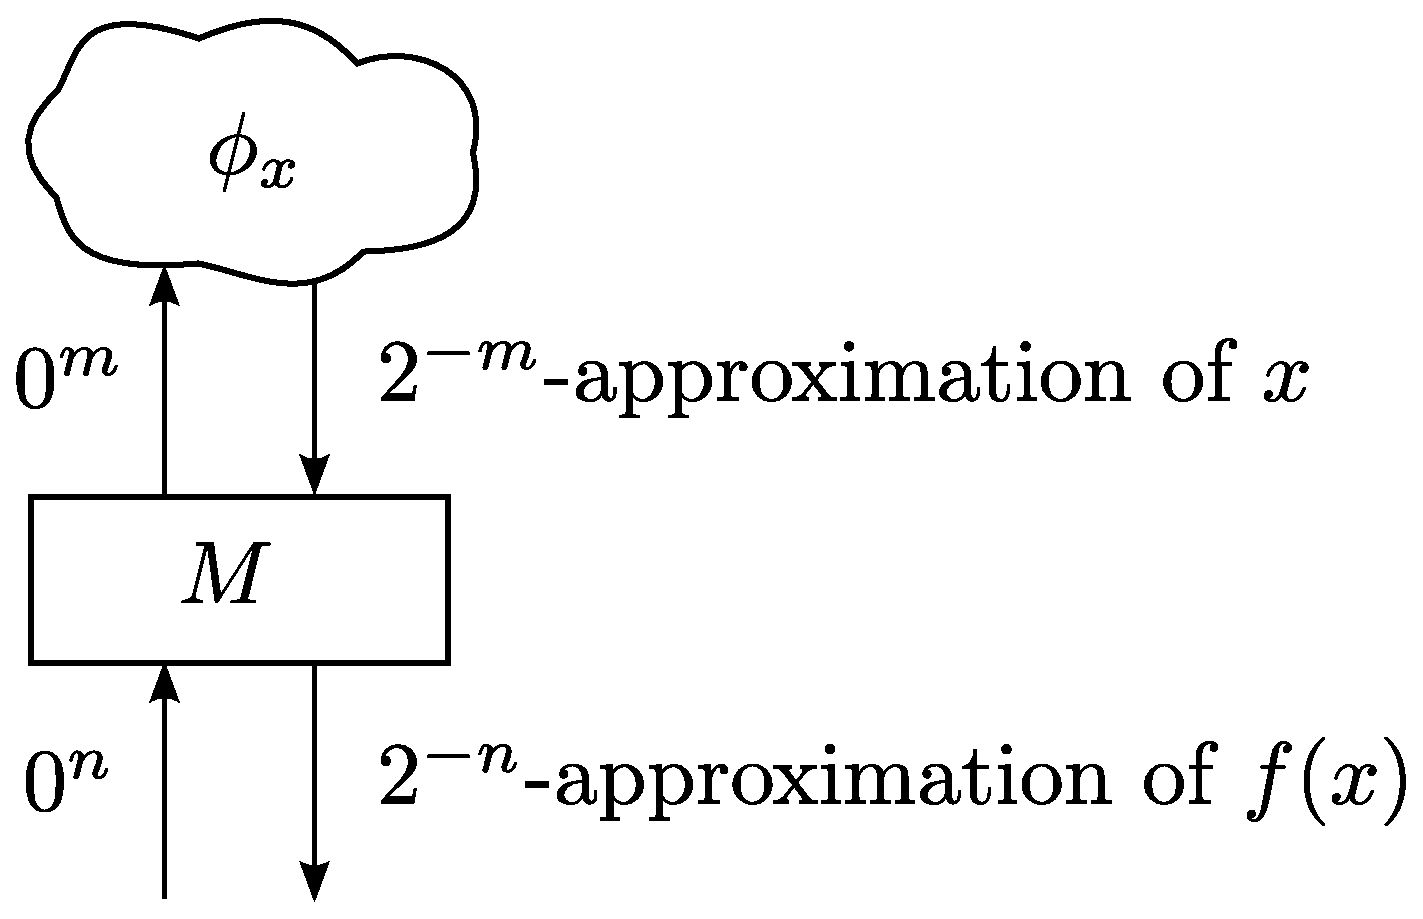
\includegraphics[height=0.17\textheight]{image/model-of-function.eps}
 \end{center}
 \caption{A machine $M$ computing a real function $f$}
 \label{fig:model-of-function}
\end{figure}

\begin{definition}
Let $A$ be a bounded closed interval of\/ $\R$.
A machine $M$ \emph{computes} a real function $f \colon A \to \R$ 
if for any $x \in A$ and any name $\phi_x$ of it,
$M^{\phi_x}$ is a name of $f(x)$.
\end{definition}

Computation of a function $f \colon A \to \R$ on
a two-dimensional bounded closed region $A \subseteq \R ^2$ 
is defined in a similar way using machines with two oracles.
A real function is (\emph{polynomial-time}) \emph{computable} if there exists some machine that computes it (in polynomial time).
Polynomial-time computability of a real function $f$ means that
for any $n \in \N$, 
an approximation of $f(x)$ with error bound $2^{-n}$
is computable in time polynomial in $n$ 
independent of the real number $x$.

By the time the machine outputs the approximation of $f (x)$ of precision~$2 ^{-n}$, 
it knows $x$ only with some precision $2 ^{-m}$.
This implies that all computable real functions are continuous.
If the machine runs in polynomial time,
this $m$ is bounded polynomially in $n$.
This implies \eqref{eq:modulus} in the following lemma, 
which characterizes polynomial-time real functions
by the usual polynomial-time computability of string functions 
without using oracle machines. 

\begin{lemma}
 \label{lem:type1representation}
 A real function is polynomial-time computable if and only if
 there exist a polynomial-time computable function 
 $\phi \colon (\Q \cap [0, 1]) \times \{0\} ^* \to \Q$ and 
 polynomial $p \colon \N \to \N$ such that
 for all $d \in \Q \cap [0,1]$ and $n \in \N$,
 \begin{equation}
  |\phi(d, 0^n) - f(d)| \le 2^{-n},
 \end{equation}
 and for all $x, y \in [0, 1]$, $n \in \N$,
 \begin{equation} 
  |x-y| \le 2^{-p(n)} \Rightarrow |f(x) - f(y)| \le 2^{-n},
   \label{eq:modulus}
 \end{equation}
where each rational number is written
as a fraction whose numerator and denominator
are integers in binary.
\end{lemma}

To talk about hardness, we define reduction. 
A language $L \subseteq \{0, 1\} ^*$ is identified with the function
$L \colon \{0, 1\} ^* \to \{0, 1\}$ such that $L (u) = 1$ when $u \in L$.

\begin{definition} \label{definition: reduction}
 A language $L$ \emph{reduces} to a function $f \colon [0, 1] \to \R$
 if there exists a polynomial-time function $S$ and a polynomial-time oracle Turing machine $M$ (Fig.~\ref{fig:reduction})
 such that for any string $u$, 
  \begin{enumerate}
   \item $S(u, \cdot)$ is a name of a real number $x_u$, and 
   \item $M^\phi(u)$ accepts if and only if $u \in L$ for any name $\phi$ of $f(x_u)$.
  \end{enumerate}
\end{definition}
This reduction may look stronger (and hence the reducibility weaker) than
the one in Kawamura~\cite{kawamura2010lipschitz} 
in that $M$ can make multiple queries adaptively, 
but this makes no difference, 
because the lengths of these queries 
are bounded by a polynomial in $\lvert u \rvert$, 
and the longest query gets all the information that any shorter query gets. 

For a complexity class~$C$, a function $f$ is \emph{$C$-hard}
if all languages in $C$ reduce to $f$.

 \begin{figure}
  \begin{center}
  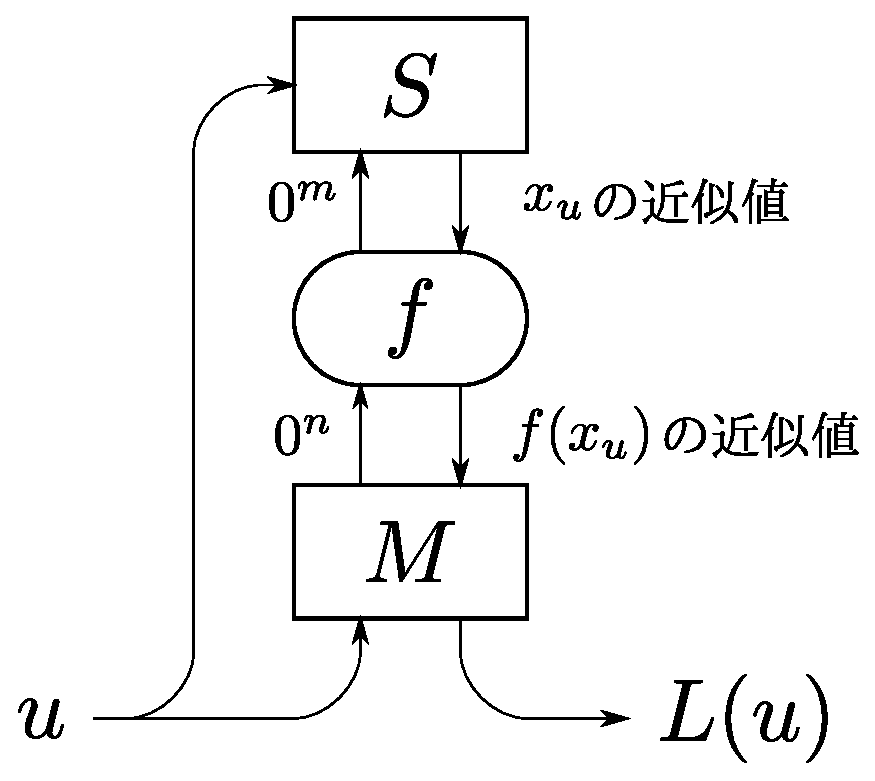
\includegraphics[scale=0.25]{image/reduction.eps}
  \caption{Reduction from a language $L$ to a function $f \colon [0,1] \to \R$}
  \label{fig:reduction}
  \end{center}
 \end{figure}


\section{連続微分可能関数と常微分方程式}
\label{section:differentiable}

基本的な証明の流れは河村によるものと等しい\cite{kawamura2010lipschitz}.
定理 \ref{DifferentiableIsPspace} の証明では,
まず任意の言語$L \in \classPSPACE$ を認識する関数族$(G_u)_u, (H_u)_u$ を得る
(補題 \ref{DIVPpolyIsPSPACEhard}).
そして $(G_u)_u, (H_u)_u$ を模倣する実関数族 $(g_u)_u, (h_u)_u$ を構成し(補題\ref{DifferentiableFamily}),
それらから定理で求める $g, h$ を構成する.
定理 \ref{KTimesIsCH} においても, ある $\classCH$ 困難な言語を認識する関数族
$(G_u)_u, (H_u)_u$ を構成し(補題 \ref{DIVPlogIsCHhard}),
それらを模倣する実関数族 $(g_u)_u, (h_u)_u$ を構成し(補題\ref{KTimesFamily}),
それらから定理で求める $g, h$ を構成する.



\subsection{差分方程式}
\label{section:divp}

定理 \ref{DifferentiableIsPspace} と定理 \ref{KTimesIsCH} の証明では,
まず滑らかな実関数の常微分方程式によって
ある種の「離散版」常微分方程式を模倣できることを示し, 
その離散版の方程式が$\classPSPACE$困難ないし$\classCH$困難であることを示す.
この節ではその離散版の方程式である「差分方程式」を定義する.

$[n] = \{0, \dots , n-1\}$ と表記する.
関数 $G \colon [P] \times [Q] \times [R] \to \{-1, 0, 1\}$ に対して,
関数 $H \colon [P + 1] \times [Q+1] \to [R]$ が
任意の $i \in [P],\ T \in [Q]$ について以下を満たすとき,
$H$ を $G$ の \emph{差分方程式} の解と呼ぶ.
\begin{gather}
   H(i, 0) = H(0, T) = 0 
\\
   H(i + 1, T + 1) = H(i+1, T) + G(i, T, H(i, T))  \label{eq:divp}
\end{gather}
$P, Q, R$ をそれぞれ\emph{段数}, \emph{列数}, \emph{欄の大きさ}と呼ぶ.
$G$ と $H$ が常微分方程式の $g$ と $h$ に対応し,
$H(i, 0) = 0$ が $h(0) = 0$ に,
式 (\ref{eq:divp}) と同値である式 $H(i + 1, T + 1) - H(i+1, T) = G(i, T, H(i, T))$
が $\D h(t) = g(t, h(t))$ と対応していると考える.

以下では文字列 $u$ ごとに差分方程式 $G _u$ を一つ定めた族 $(G _u) _u$ を考える. 
各 $u$ に対して $G_u$ の段数と列数, 解をそれぞれ $P_u, Q_u, H_u$ としたとき,
言語 $L$ がこの族 $(G_u)_u$ によって認識されるとは,
$H_u(P_u, Q_u) = L(u)$ を満たすこととする(表 \ref{fig:divp}).
ここで言語 $L \subseteq \{0, 1\} ^*$ は
関数 $L \colon \{0, 1\} ^* \to \{0, 1\}$ と同一視し, 
$u \in L$ のとき $L (u) = 1$ としている. 

 \begin{figure}
  \label{fig:divp}
  \begin{center}
   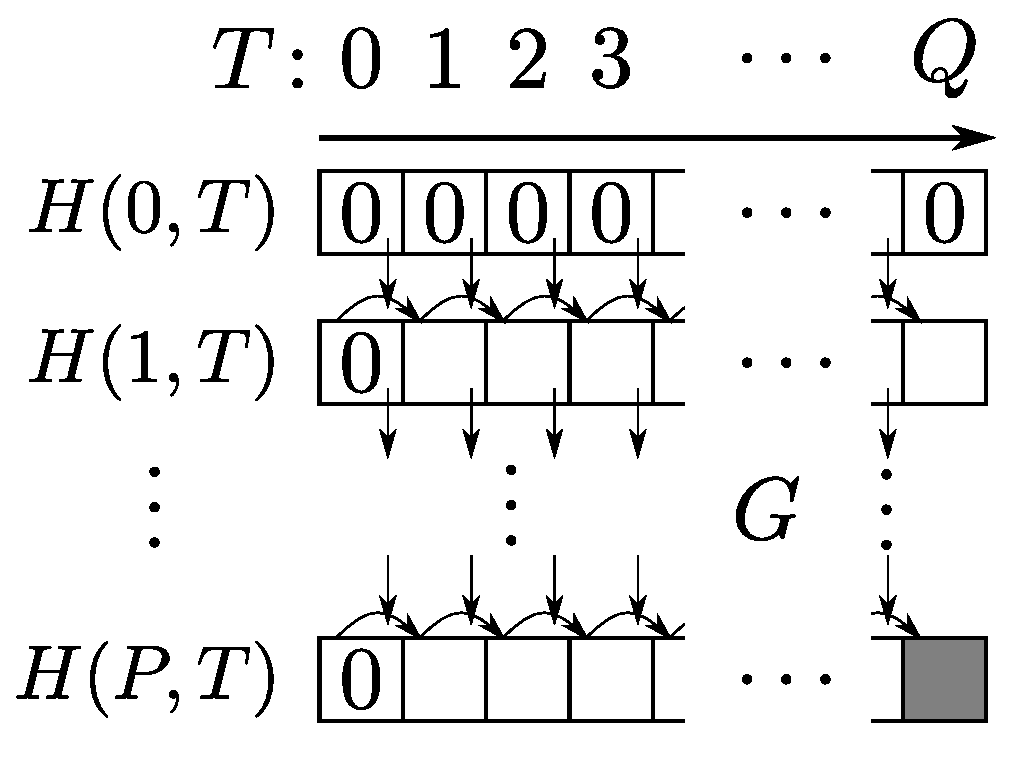
\includegraphics[height=0.2\textheight]{image/divp.eps}
  \end{center}
  \caption{差分方程式と認識される言語}
 \end{figure}

$(G_u)_u$ が{\bf 一様}であるとは,
各 $u$ について $G _u$ の段数, 列数及び欄の大きさが $|u|$ の多項式の指数($2^{\mathrm{poly} (|u|)}$)で抑えられ, 
かつ与えられた $(u, i, T, Y)$ から多項式時間で $G_u(i, T, Y)$ が
計算できることと定義する.

$G_u$ の段数がさらに $|u|$ の多項式, 対数で抑えられるとき, 
族 $(G_u) _u$ はそれぞれ\emph{多項式段}, \emph{対数段}であるという. 
河村の論文では次が示されている.

\begin{lemma}[補題 4.7 \cite{kawamura2010lipschitz}]
 \label{DIVPpolyIsPSPACEhard}
 任意の言語 $L \in \classPSPACE$ に対して,
 その言語を認識する多項式段一様関数族が存在する.
\end{lemma}

$(\infty, 1)$ 回微分可能な関数の常微分方程式においても,
この補題を用いて$\classPSPACE$困難な常微分方程式の解を構成する.

2回以上微分可能な関数の常微分方程式の複雑さを考えるとき,
その滑らかさによる制限により多項式段の差分方程式を模倣することはできなかった.
しかし差分方程式を対数段に制限してやれば模倣可能であり,
対数段一様な関数族によって認識される言語の困難性が重要である.

\begin{lemma}
 \label{DIVPlogIsCHhard}
 $\classCH$ 困難で対数段一様な関数族によって認識される言語が存在する.
\end{lemma}

補題 \ref{DIVPpolyIsPSPACEhard} が$\classPSPACE$の任意の言語について述べているのに対して,
この補題は$\classCH$困難な或る言語について述べているという違いがある.
しかし定理の証明において必要なのは言語クラスに対して困難な或る言語を認識できることであり,
補題 \ref{DIVPpolyIsPSPACEhard} を補題 \ref{DIVPlogIsCHhard} と同じ形式
($\classPSPACE$ 困難で多項式段一様な関数族によって認識される言語が存在する)
に変えても定理を証明するには十分である.


\subsection{計数階層と対数段差分方程式}
\label{subsection: counting hierarchy}

\emph{計数階層}(Counting Hierarchy($\classCH$)) とは
Wagner によって導入された計算量クラスである\cite{wagner1986complexity}.
多項式階層({\bf PH})が {\bf NP} の神託機械を用いて,
\begin{align*}
 \Sigma^p_0 
 &= \classP \\
 \Sigma^p_{k+1}
 &= \mathbf{NP}^{\Sigma^p_k}
\end{align*}
\[
 \mathbf{PH} = \bigcup_k \Sigma^p_k
\]
と定義されるのに対し,
計数階層は多項式階層の {\bf NP} を {\bf PP} で置き換えたものである. つまり
\begin{align*}
 \C_0 \classP  
 &= \classP \\
 \C_{k+1} \classP
 &= \classPP^{\C_k \classP}
\end{align*}
\[
 \classCH = \bigcup_k \C_k \classP.
\]
上記の特徴付けは Tor{\'a}n によるものであり,
Wagner によるオリジナルの定義とは異なる\cite{toran1991complexity}.

$\mathbf{PH} \subseteq \classCH \subseteq \classPSPACE$ だが,
$\mathbf{PH} = \classCH$, $\classCH = \classPSPACE$
か否かは未解決である.

Wagner によって $\classCH$ の各階層 $\C_n \classP$ に対してそれぞれ完全問題が存在することが示されている\cite{wagner1986complexity}.
量化子 $\C$ を自然数 $m$, 論理式 $A(x_1, \dots, x_l)$, 
$l$ 個の論理変数の組 $\alpha$ について以下のように定義する.
\begin{equation}
 \C^m \alpha A(\alpha) 
  \longleftrightarrow 
  \Bigl|\{\alpha \in \{0,1\}^l \mid A(\alpha) = 1\}\Bigr| \ge m.
\end{equation}
$\C^1 = \exists$, $\C^{2^l} = \forall$ であり, $\C$ は $\exists, \forall$ の
一般化と言える.
言語 $\C_n B_{be}$ を以下のように定義する.
\begin{equation}
 \langle \phi(x_1, \dots, x_n), m_1, \dots, m_n \rangle \in \C_n B_{be}
 \longleftrightarrow
 \C^{m_1}{\alpha_1} \cdots \C^{m_n}{\alpha_n} \phi(\alpha_1, \dots, \alpha_n) 
\end{equation}

ただし $\langle y_1, \dots, y_i \rangle$ は組み合わせ関数,
$x_i$, $\alpha_i$ は $l_i$ 個の論理変数の組,
$\phi(x_1, \dots, x_n)$は$x_1, \dots, x_n$のみを変数として持つ論理式とする.


\begin{lemma}[Theorem 7 \cite{wagner1986complexity}] \label{lemma:CnP-complete}
 $\C_n B_{be}$ は $\C_n\classP$ 完全.
\end{lemma}


各 $\C_n B_{be}$ をまとめた言語 $\C_{\log} B_{be}$ を以下のように定義する.
\begin{equation}
 \langle 0^{2^n}, u \rangle \in \C_{\log} B_{be}
 \longleftrightarrow
 u \in \C_n B_{be}
\end{equation}
この $\C_{\log} B_{be}$ が補題 \ref{DIVPlogIsCHhard} で求める言語であること,
つまり$\classCH$困難かつ対数段一様関数族によって認識可能であることを示す.


\begin{proof}[\rm 補題 \ref{DIVPlogIsCHhard} の証明]
 $\C_{\log} B_{be}$が$\classCH$困難であることを示す.
 任意の $\classCH$ の言語 $A$ はある階層 $\C_n \classP$ に属する. 
 補題 \ref{lemma:CnP-complete} より任意の $u \in \{0,1\}^*$ について
 $u \in A \leftrightarrow f(u) \in \C_n B_{be}$ 
 を満たす多項式時間関数 $f$ が存在する.
 \begin{align}
  u \in A 
  & \longleftrightarrow \langle 0^{2^n}, f(u) \rangle \in \C_{\log} B_{be}
 \end{align}
 $n$ は定数であるため $\langle 0^{2^n}, f(\cdot) \rangle$ は多項式時間関数.
 よって $A$ は $\C_n B_{be}$ に多項式時間還元可能.


 $\C_{\log} B_{be}$を認識する関数族 $(G_u)_u$, 
 その解$(H_u)_u$, 関数 $p \colon \N \to \N$, 多項式 $q,r$ を構成する.
 自然数 $n, m_1, \dots, m_n$, 論理式$\phi$を
 $u  = \langle 0^{2^n}, 
 \langle \phi(x_1, \dots, x_n), m_1, \dots, m_n \rangle \rangle$
 を満たすものとする. 
 (そのような$n, m_1, \dots, m_n, \phi$が存在しないとき$u \not \in A$.)
 
 
 $L = C_{\log} B_{be}$,
 $l_i = |x_i|$,
 $s_i = \sum^i_{j=1}l_j + 2i$  と表記する.
 関数 $C^m \colon \N \to \{0,1\}$ を
 \begin{equation}
  C^m(Y) 
     = \begin{cases}
       1 & (Y \ge m) \\
       0 & (Y < m) \end{cases}
 \end{equation}
 と定義する. 
 任意の $i = 0, \dots, n$ と $n-i$ 個の文字列 
 $\beta_{i+1} \in \{0,1\}^{l_{i+1}}, \dots, \beta_n \in \{0,1\}^{l_n}$ 
 について論理式
 $\C^{m_{i}}{\alpha_i} \cdots \C^{m_1}{\alpha_1}
 \phi(\alpha_1, \dots, \alpha_i, \beta_{i+1}, \dots, \beta_n)$
 の真偽値を $\phi_i(\beta_{i+1}, \dots, \beta_n)$ と表記する.
 \begin{align}
  \phi_0 (\beta_1, \dots, \beta_n) &= \phi(\beta_1, \dots, \beta_n)
  \\ \label{eq:phi-step}
  \phi_{i+1}(\beta_{i+2}, \dots, \beta_n) 
  &= C^{m_{i+1}}\left(\sum\nolimits_{\alpha_i \in \{0,1\}^{l_i}} 
  \phi_i(\alpha_{i+1}, \beta_{i+2}, \dots, \beta_{n})\right) 
  \\
  \phi_n() &= L(u) 
 \end{align}
 $T \in \N$ に対し, $T_i$ を $T$ の2進表記における $i$ 桁目, 
 $T_{[i,j]} = T_{j-1} T_{j-2} \cdots T_{i+1} T_{i}$ と表記する.


 $G_u$ を $(i, T, Y) \in [n+1] \times [2^{s_n}+1] \times [2^{|u|}]$ の範囲で
 を以下のように定義する. 一段目つまり $i=0$ ならば
 \begin{equation}
  G_u(0,T,Y) = 
   (-1)^{T_{s_1}}\phi(T_{[1,s_1]}, T_{[s_1+1,s_2]},
    \dots, T_{[s_{n-1}+1,s_n]}) 
 \end{equation}
 $i \ge 1$ ならば
 \begin{equation} \label{eq:def-Gu:case0}
  G_u(i,T,Y) = 
   \begin{cases}
    (-1)^{T_{s_{i+1}}} C^{m_i}(Y) 
    & (T_{[1,s_i]} = 10 \cdots 0) \\
    0 & (\text{othewise}).
   \end{cases} 
 \end{equation}


 任意の $i \in [n+1]$, $T \in [2^{s_n}+1]$ について,
 $H_u(i,T) \in [2^{l_i}+1]$ が成りたつこと,
 および $T_{[1,s_i]} = 10 \cdots 0$ ならば
 \begin{equation} \label{eq:subformula}
  G_u(i,T,H_u(i,T)) = (-1)^{T_{s_{i+1}}} 
   \phi_i(T_{[s_i+1, s_{i+1}]}, \dots, T_{[s_{n-1}+1, s_n]})
 \end{equation}
 を満たすことを $i$ についての帰納法により示す.
 上記が成り立つとき,
 $i=n$, $T=2^{s_n}$ において $G_u(n, 2^{s_n}, H_u(n,2^{s_n})) = \phi_n() = L(u)$
 よって $H_u(n+1, 2^{s_n}+1) = L(u)$.
 ここで 
 \begin{gather}
  n+1 \le \log(|0^{2^n}|) + 1 = O(\log(|u|)) \\
  2^{s_n}+1 \le 2^{s_n+1} \le 2^{|u|}
 \end{gather}
 より $p(u) = n+1, q(x) = r(x) = x$ とおき $G_u$ を
 $[p(u)] \times [2^{q(|u|)}] \times [2^{r(|u|)}]$ の範囲に拡張すると
 $H_u(p(u), 2^{q(|u|)}) = L(u)$.

 $i=0$ のとき, 式(\ref{eq:def-Gu:case0})より成り立つ.
 $i=j$ のとき, 成り立つと仮定する, $Y = H_u(i+1, T)$ とおくと
 \begin{align}
  Y 
  &= \sum_{V = 1}^{T-1} G_u(i, V, H_u(i, V)) \\
  &= \sum (-1)^{V_{s_{i+1}}} \phi_i(V_{[s_i+1, s_{i+1}]}, 
   \dots, V_{[s_{n-1}+1, s_n]})
 \end{align}
 $T_{[1, s_{i+1}]} = 10 \cdots 0$ のとき,
 $V_{[1, s_n]} = T_{[s_{i+1}+1,s_n]} 0 \alpha 1 0 \cdots 0$ であるとき
 以外の値は打ち消し合うので,
 \begin{equation}
  Y = \sum\nolimits_{\alpha \in \{0,1\}^{l_i}} 
  \phi_i(\alpha, T_{[s_{i+1}+1, s_{i+2}]}, \dots, T_{[s_{n-1}+1, s_n]})
 \end{equation}
 式(\ref{eq:phi-step})より
 \begin{align}
  G_u(i+1,T,H_u(i+1,T)) 
  &= (-1)^{T_{s_{i+2}}} C^{m_{i+1}} (Y)\\
  &= (-1)^{T_{s_{i+2}}} \phi_{i+1}(T_{[s_{i+1}+1, s_{i+2}]}, \dots, T_{[s_{n-1}+1, s_n]})
 \end{align}
 よって $i=j+1$ でも成り立つ.
 \end{proof}



\subsection{差分方程式を模倣する関数族}

\begin{lemma}
 \label{DifferentiableFamily}
 任意の言語 $L \in \classPSPACE$ に対して, 
 二変数多項式 $\mu$ が存在して,
 任意の多項式 $\gamma$ に対して,
 多項式 $\rho$, 実関数族 $(g_u)_u, (h_u)_u$ で, 
 $(g_u)_u$ は多項式時間計算可能であり,
 各文字列 $u$ に対して以下を満たすものが存在する.
 \begin{enumerate}
  \item $g_u\colon [0,1] \times [-1,1]\to \R$, $h_u\colon [0,1] \to [-1,1]$;
  \item $h_u$ は $g_u$ の常微分方程式 (\ref{eq:ode}) の解; 
  \item $g_u$ は $(\infty, 1)$ 回連続微分可能;
  \item 任意の $i \in \N$, $y \in [-1,1]$ に対して
	\begin{equation*}
	 \D ^{(i, 0)} g_u(0,y) = \D ^{(i, 0)} g_u(1,y) = 0;
	\end{equation*}
  \item \label{enum:infty1}
	任意の $i \in \N$, $j \in \{0,1\}$ に対して
	\begin{equation*}
	 |\D ^{(i,j)} g_u| \leq 2^{\mu(i, |u|) - \gamma(|u|)};
	\end{equation*}
  \item $h_u(1) = 2^{-\rho(|u|)}L(u)$.
 \end{enumerate}
\end{lemma}


 \begin{lemma}
  \label{KTimesFamily}
  任意の自然数 $k \ge 2$ に対して,
  $\classCH$ 困難な言語 $L$,
  二変数多項式 $\mu$ が存在して,
  任意の多項式 $\gamma$ に対して,
  関数 $\rho \colon \N \to \N$, 関数族 $g_u, h_u$ で,
  $\rho, (g_u)_u$ は多項式時間計算可能であり,
  各文字列 $u$ に対して以下を満たすものが存在する.
  \begin{enumerate}
   \item $g_u\colon [0,1] \times [-1,1]\to \R, \quad h_u\colon [0,1] \to [-1,1]$;
   \item $h_u$ は $g_u$ の常微分方程式 (\ref{eq:ode}) の解;
   \item $g_u$ は $(\infty, k)$ 階連続微分可能;
   \item \label{enum:boundary}
	 任意の $i \in \N$, $y \in [-1,1]$ に対して
	 \begin{equation*}
	  \D^{(i, 0)} g_u(0,y) = \D^{(i, 0)} g_u(1,y) = 0 ;
	 \end{equation*}
   \item \label{enum:inftyk}
	 任意の $i \in \N$, $j \in \{0, \dots, k\}$ に対して
	 \begin{equation*}
	  \left|\D^{(i,j)} g_u(t,y)\right| \le 2^{\mu(i, |u|) - \gamma(|u|)};
	 \end{equation*}
   \item $h_u(1) = 2^{-\rho(|u|)}L(u)$.
  \end{enumerate}
 \end{lemma}


 この補題より各 $h_u$ が $g_u$ の常微分方程式の解であり, 
 $h_u(1)$ に $L(u)$ の情報を持つ
 実関数族 $(g_u)_u, (h_u)_u$ の存在が示される.
 河村によるLipschitz連続な常微分方程式の$\classPSPACE$困難性の証明における,
 補題 4.1 に対応するが,
 $g$ を微分可能にするため, 条件 (iii) -- (v) が付け加えられている.
 

 この補題の証明の基本的な流れを説明する.
 任意の言語 $L \in \classPSPACE$ に対し, 
 補題 \ref{DIVPpolyIsPSPACEhard} を用いて $L$ を認識する $(G_u)_u$ 
 及びその差分方程式の解 $(H_u)_u$ を得る.
 そして各 $G_u, H_u$ を模倣する
 滑らかな $g_u \colon [0,1] \times [-1, 1] \to \R$ 
 とその常微分方程式の解 $h_u \colon [0,1] \to \R$ を構成する.
 また $(G_u)_u$ の一様性から $(g_u)_u$ の多項式時間計算可能性を示す.


 上記の証明は基本的に, Lipschitz条件の場合と変わらない.
 異なる点は, $g_u$ を滑らかな関数にするため, 
 以下のような無限回微分可能な多項式時間実関数 $f \colon [0,1] \to \R$ を用いて
 $g_u$ を構成していることである.

 \begin{lemma}[補題 3.6 \cite{ko1991complexity}]
  \label{SmoothFunction}
  以下を満たす多項式時間計算可能で無限回微分可能な
  実関数 $f \colon [0,1] \to \R$ が存在する.

  \begin{enumerate}
   \item $f(0) = 0, \quad f(1) = 1$;
   \item 任意の $n \ge 1$ で $f^{(n)}(0) = f^{(n)}(1) = 0$;
   \item $f$ は $[0,1]$ で単調増加;
   \item 任意の $n \ge 1$ で $\D^n f$ は多項式時間実関数.
  \end{enumerate}
 \end{lemma}

 さらにここでは上記の条件に加えて, 
 \begin{enumerate}
  \setcounter{enumi}{4} 
  \item 以下を多項式 $s$が存在
	\begin{equation} \label{enum:polynomial-size}
	 |\D^n f| \le s(n)
	\end{equation}
 \end{enumerate}
 を満たすような$f$が存在することを用いて証明する.

 補題 \ref{DifferentiableFamily} の証明はLipschitzの場合とほとんど変わらず,
 細かな差異も補題 \ref{KTimesFamily} の証明に含まれるものと同じであるため省略する.

 \begin{proof}[\rm 補題 \ref{KTimesFamily} の証明]
  補題 \ref{DIVPlogIsCHhard} より
  $\classCH$ 困難な言語 $L$ を認識する
  対数段一様関数族 $(G_u)_u$, その解 $(H_u)_u$, 
  $P_u = p(|u|), Q_u = 2^{q(|u|)}, R_u = 2^{r(|u|)}$ を満たす関数$p$, 
  多項式 $q,r$ を得る.
  さらに以下のように仮定する.
  \begin{equation}
   H_u(i, 2^{q(|u|)}) = \begin{cases}
			L(u) & (i=p(|u|)) \\
			0 & (i<p(|u|)).
			\end{cases}
  \end{equation}

 $B = 2^{\gamma(|u|) + r(|u|) + s(k) + k + 3}$ とおき, 
 各 $(t, y) \in [0,1] \times [-1, 1]$ に対して,
 自然数 $N$, $\theta \in [0,1]$, 整数 $Y$, $\eta \in [-1/4, 3/4]$ を
 $t = (T + \theta)2^{-q(|u|)}$, $y = (Y + \eta)B^{-(k+1)^{j_u(T)}}$ を満たすように
 定める.
 
 そのとき,
 \begin{equation}
  \delta_{u, Y} (t) = \frac{2^{q(|u|)} \D f(\theta)}{B^{(k+1)^{j_u(T)+1}}} 
   G_u\left( j_u(T),\ T,\ Y \bmod 2^{r(|u|)} \right)
 \end{equation}
 とおき $g_u, h_u$ を以下のように定義する.
 \begin{equation}
  \label{eq:gu}
  g_u(t,y) 
  = \begin{cases}
     \delta_{u, Y}(t)
     & (\eta \le \frac 1 4)
     \\
     ( 1-f ( \frac{4\eta-1}{2})) \delta_{u, Y}(t) 
     + f ( \frac{4\eta-1}{2}) \delta_{u,Y+1}(t)
     & (\eta > \frac 1 4)
    \end{cases}
 \end{equation}
 \begin{equation} 
  h_u(t) 
   = \sum^{p(|u|)}_{i=0} \frac{H_u(i, T)}{B^{(k+1)^i}}  
  + \frac{f(\theta)}{B^{(k+1)^{j_u(T)+1}}} G_u(j_u(T), T, H_u(j_u(T), T)) 
  \label{eq:hu}
 \end{equation}
  ただし$f$と多項式$s$は補題 \ref{SmoothFunction}
  および式(\ref{enum:polynomial-size})を満たすものとする.


 上記のように定義した $g_u, h_u$ が補題\ref{DifferentiableFamily} で求める
 性質を満たすことを示す. (i) は自明. 
 $(g_u)_u$ が多項式時間計算可能であることは
  補題 \ref{lem:type1representation}によって示される.


 $h_u$ は $g_u$ の常微分方程式の解であることを示す.
 任意の $t$ について $h_u(t) = (Y + \eta) B^{-j_u(T)}$ を満たす 
 $\eta \in [-1/4, 1/4]$ が存在する. 
 つまり常微分方程式の解$h$は式 $\ref{eq:gu}$ の一つ目の場合のみを考慮すればよい.
 \begin{equation}
  Y = \sum_{i=0}^{j_u(T)} \frac{H_u(i, T)}{B^{(k+1)^i}} \cdot B^{(k+1)^{j_u(T)}}.
 \end{equation}
 $B$ は $2^{r(|u|)}$ の倍数なので,  $Y \bmod 2^{r(|u|)} = H_u(j_u)$. 
 $g_u$ に代入すると,
 \begin{align*}
   g_u(t, h_u(t)) 
  & =  \frac{2^{q(|u|)} \D f(\theta)}{B^{(k+1)^{j_u(T)+1}}}
   G_u(j_u(T), T, H_u(j_u(T), T)) \\
  & =  \D h_u(t).
 \end{align*}
 よって $h_u$ は $g_u$ の常微分方程式の解.

  $g_u$ が $(\infty, k)$ 階連続的微分可能であることを示す.
  $\eta$ が $[-1/4, 1/4]$ と $[1/4, 3/4]$ である区間それぞれにおいて微分する.
  任意の $i \in \N$ について

  \begin{equation}
   \D^i \delta_{u,Y}(t) 
    = \frac{2^{(i+1)q(|u|)} \D^{i+1}f(\theta)}{B^{(k+1)^{j_u(T)+1}}}
    G_u\left( j_u(T),\ T,\ Y \bmod 2^{r(|u|)} \right)
  \end{equation}

  \begin{equation}
   \label{eq:derivativeofgu}
    \D^{(i,0)} g_u(t, y)
     = \begin{cases}
 	\D^i \delta_{u, Y}(\theta) 
	\hfill (- \frac 1 4 < \eta < \frac 1 4) \\
	\left( 1-f \left(\frac{4\eta-1}{2}\right)\right) 
	\D^i \delta_{u, Y}(\theta) 
	+ f \left(\frac{4\eta-1}{2}\right) \D^i \delta_{u,Y+1}(\theta) \\
	\hfill (\frac 1 4 < \eta < \frac 3 4)
       \end{cases}
  \end{equation}   
  $j \in \{1, \dots , k\}$ について,

  \begin{equation}
    \D^{(i,j)} g_u(t, y)
     = \begin{cases}
	0 \hfill (- \frac 1 4 < \eta < \frac 1 4) \\
	(2B^{(k+1)^{j_u(T)}})^j \D^j f(\frac{4\eta - 1}2)
	(\D^i \delta_{u,Y+1}(\theta)-\D^i \delta_{u, Y}(\theta)) \\
	\hfill (\frac 1 4 < \eta < \frac 3 4)
       \end{cases}
  \end{equation}
  境界においても連続であるため,
  $g_u$ は $(\infty, j)$ 階連続的微分可能であることが示された.
  式 (\ref{eq:derivativeofgu}) に $t = 0, 1$ ($\theta = 0$) を代入して
  $\D^{(i, 0)} g_u(0,y) = \D^{(i, 0)} g_u(1,y) = 0$.
  上記の式より, $\mu(x, y) = (x+1)q(y) + s(x+1)$とおくと,
  任意の $i \in \N$, $j \in \{0, \dots, k\}$ について
  $|\D^{(i,j)} g_u| \leq 2^{\mu(i, |u|) - \gamma(|u|)}$.

 \begin{align*}
  h_u(1) &= \frac{H_u(p(|u|), 2^{q(|u|)})}{B^{2^{p(|u|)}}}  \\
  &= L(u) \cdot 2^{-2^{p(|u|)} \cdot (\gamma(|u|) + r(|u|) + 3) } \taghere
 \end{align*}
 より, $\rho(x) = 2^{p(x)} \cdot (\gamma(x) + r(x) + 3)$ とおくと成り立つ.
 \end{proof}


 補題 \ref{DifferentiableFamily} の証明では
 $\classPSPACE$困難な言語を認識する多項式段一様関数族$(G_u)_u$とその解$(H_u)_u$に対して
 \begin{align}
  \delta_{u, Y} (t) &= \frac{2^{q(|u|)} \D f(\theta)}{B^{{j_u(T)+1}}} 
   G_u\left( j_u(T),\ T,\ Y \bmod 2^{r(|u|)} \right)
  \\
  g_u(t,y) 
  &= \begin{cases}
     \delta_{u, Y}(t)
     & (\eta \le \frac 1 4)
     \\
     ( 1-f ( \frac{4\eta-1}{2})) \delta_{u, Y}(t) 
     + f ( \frac{4\eta-1}{2}) \delta_{u,Y+1}(t)
     & (\eta > \frac 1 4)
    \end{cases}
  \\
  h_u(t) &= \sum^{p(|u|)}_{i=0} \frac{H_u(i, T)}{B^{i}}  
  + \frac{f(\theta)}{B^{{j_u(T)+1}}} G_u(j_u(T), T, H_u(j_u(T), T)) 
 \end{align}
 と定める.
 $(g_u)_u$と$(h_u)_u$が補題 \ref{DifferentiableFamily} で求める性質を満たすことは,
 補題 \ref{KTimesFamily} の証明と同様に示される.


\subsection{主定理の証明}

 主定理の証明はLipschitzの場合とほぼ同じである.
 補題 \ref{DifferentiableFamily} から得られる
 $(g_u)_u$ と $(h_u)_u$ から滑らかな $g$ と
 その常微分方程式の解 $h$ を構成する.
 各 $h_u(1)$ には $L(u)$ の情報が含まれるため,
 すべての $h_u$ を一つの関数 $h$ に埋め込みたい.
 そこで [0,1] を無限の区間に分割し, $h$ の各文字列 $u$ に対応する区間
 $[l^-_u, c_u]$ に $h_u$ を
 縮小して埋め込む. 
 ただし次の文字列 $u'$ の計算に影響を与えないために,
 $h_u$ を定義域方向について反転したものを
 区間 $[c_u, l^+_u]$ に埋め込むことで影響を相殺する.
 つまり $h(l^-_u) = 0,\ h(c_u) = 2^{-\rho'(|u|)} L(u),\ h(l^+_u) = 0$ を満たす
 ように $h_u(t)$埋め込む.
 ただし $\rho'$ とは $\rho$ に縮小率をかけたものとする.
 同様に $g$ は $h$ が常微分方程式の解となるよう,
 各文字列 $u$ に対応する区間に $g_u$ を縮小して埋め込む.

 定理 \ref{DifferentiableIsPspace} と定理 \ref{KTimesIsCH} の関係は
 補題 \ref{DifferentiableFamily} と補題 \ref{KTimesFamily} の関係と等しい.
 つまり $\classPSPACE$ が $\classCH$ に置き換わり,
 $(\infty, 1)$ 回連続微分可能が $(\infty, k)$回連続微分可能に一般化されている.
 よって定理 \ref{KTimesIsCH} の証明から
 定理 \ref{DifferentiableIsPspace} の証明が構成できる.

\begin{proof}[\rm 定理 \ref{KTimesIsCH} の証明]
 $L$ を $\classCH$ 困難な言語とおく.
 $L$ に対して補題 \ref{DifferentiableFamily} を用いて,
 まず多項式 $\mu$ をえる.
 \begin{align}
  \lambda(x) &= 2x + 2,&
  \gamma(x) &= x\mu(1, x) + x \lambda(x)
 \end{align}
 とおき, 各 $u$ に対して 
\begin{align}
 \Lambda_u 
 &= 2^{\lambda(|u|)}, &
 c_u 
 &= 1-\frac{1}{2^{|u|}}+\frac{2\bar{u}+1}{\Lambda_u}, &
 l_u^\mp 
 &= c_u\mp\frac{1}{\varLambda_u} 
\end{align}  
 とおく. ただし $\bar u \in \{0, \dots, 2^{|u|} - 1\}$ は $u$ を二進数と
 して解釈した数.
 $\gamma$ に対して, 補題より $\rho$, $(g_u)_u$, $(h_u)_u$ を得る.


 任意の $[0,1)$ の実数に対して,
 $l^\mp_u \pm \frac{t}{\Lambda_u}$ がその実数と等しくなるような
 $u, \pm, t\in [0,1]$ が存在する.
 関数 $g, h$ を $t \in [0,1)$, $y \in [-1, 1]$ に対して,
 \begin{align}
 g \left(l^\mp_u \pm \frac{t}{\Lambda_u}, \frac{y}{\Lambda_u}\right)
  &= \begin{cases}
      \pm \displaystyle \sum_{l=0}^k \frac{\D^{(0,l)}g_u(t,1)}{l!} (y-1)^l 
      &  (1<y) \\
      \pm g_u(t, y)      & (-1 \le y \le 1) \\
      \pm \displaystyle \sum_{l=0}^k \frac{\D^{(0,l)}g_u(t,-1)}{l!} (y+1)^l  
      &  (1<y) \\
    \end{cases} 
  \\
 h \left( l^\mp_u \pm \frac{t}{\Lambda_u} \right) 
  & = \frac{h_u(t)}{\Lambda_u}.
\end{align}
 $t=1$のとき $g(1,y) = 0$, $h(1) = 0$ と定義する.


 この $g$ と $h$ が定理 \ref{DifferentiableIsPspace} で求める関数
 の性質を満たすことを示す.


 
 まず $g$ が多項式時間計算可能であることを
 補題 \ref{lem:type1representation} を用いて示す.
 各有理数 $T,Y$ について $g(T, Y)$ を求めるとき,
 $T=l_u^\mp \pm t/\Lambda_u$, $Y = y/\Lambda_u$ を満たすような
 $u, \pm, t, y$ は, 多項式時間で計算可能であり,
 $(g_u)_u$ は多項式時間計算可能なので $g(T, Y)$ は多項式時間計算可能.


 $g$ が $(\infty, k)$ 回連続的微分可能であることを示す.
 $g_u$ は $(\infty, k)$ 階連続的微分可能であるため,
 各区間においては$(\infty, k)$ 階連続的微分可能である.
 $i \in \N$, $j \in \{0, \dots, k\}$, $t \in (0, 1)$ において
\begin{equation}
   \D^{(i, j)}g \left(l^\mp_u \pm \frac{t}{\Lambda_u}, \frac{y}{\Lambda_u}\right)
   = \begin{cases}
      \pm \Lambda_u^{(i, j)} \sum^{k}_{l=j} \frac{\D^{(i,l)} g_u(t,1)}{(l-j)!}
      (y - 1)^l &  (1<y)
      \\
      \pm \Lambda_u^{(i,j)} \D^{(i, j)} g_u(t, y) & (-1 < y < 1)
      \\
      \pm \Lambda_u^{(i, j)} \sum^{k}_{l=j} 
      \frac{\D^{(i,l)} g_u(t, -1)}{(l-j)!} (y + 1)^l &  (1<y)
    \end{cases}
\end{equation}
 $\D^{(i,j)}g_u$ は連続であるため 
 $t \in (0,1)$, $y \not = -1, 1$ の区間において連続.
 境界($t = 0, 1$または$y = -1, 1$)において連続であることは,
 定義および補題 \ref{KTimesFamily}(\ref{enum:boundary})によりしめされる.
 第一変数が $1$ へ向かうとき
 \begin{align*}
  \left|\D^{(i, j)}g \left(l^\mp_u \pm \frac{t}{\Lambda_u},
  \frac{y}{\Lambda_u}\right)\right|
  &\le 
  \Lambda_u^{i+j} \sum^{k}_{l=j} \left(|\D^{(i,l)} g_u |(\Lambda_u + 1)^l \right)
  \\
  & \le \Lambda_u^{i+j+k}  2^{k + \mu(i, |u|) - \gamma(|u|)}
  \\
  & =  2^{(i+j+k)\lambda(|u|) + k + \mu(i, |u|)  - \gamma(|u|)}.  \taghere
  \label{eq:sizeofderivative}
 \end{align*}
 $\gamma$ のとり方により, $|u| \to \infty$ のとき 
 式 (\ref{eq:sizeofderivative}) は 0 に収束する.
 よって  $\lim_{t \to 1-0}\D^{(i,j)} g(t,y) = g(1, y) = 0$.
 以上により $g$ が $(\infty, k)$ 階連続的微分可能.
 

 $h$が$g$の常微分方程式の解であることを示す. 
 $h(0)=0$, 
 \begin{equation}
  \D h \left( l^\mp_u \pm \frac{t}{\Lambda_u} \right)
  = \pm \frac{\D h_u(t)}{\Lambda_u} = \pm g_u \left(t, h_u(t)\right) 
  = g\left(l^\mp_u \pm \frac{t}{\Lambda_u}, 
	h\left(l^\mp_u \pm \frac{t}{\Lambda_u}\right) \right).
\end{equation}


 $L$ は $h$ に還元可能であることを示す.
 \begin{equation}
  h(c_u) = \frac{h_u(1)}{\Lambda_u}
   = \frac{L(u)}{2^{\lambda(|u|)+\rho(|u|)}}
 \end{equation}
 つまり $R,S,T$ を以下のように定義することで, 還元可能.
 \begin{align}
  R(u,v) &= v \\
  S(u, 0^n) &= \lfloor 2^nc_u \rfloor \text{を表す文字列,} \\
  T(u) &= 0^{\lambda(|u|)+\rho(|u|)}
 \end{align}
 $L$ は $\classCH$ 困難であるため, $h$ は $\classCH$ 困難.
\end{proof}


%%% 証明は削除, master に残っているものを後でマージする.

\section{Other Versions of the Problem}

\subsection{Complexity of the Final Value}
\label{section: final value}
In the previous section, 
we considered the complexity of the solution~$h$ of the ODE as a real function. 
Here we discuss the complexity of the final value $h (1)$ and
relate it to tally languages (subsets of $\{0\}^*$), 
as did 
Ko~\cite{ko1983computational} and 
Kawamura~\cite[Theorem~5.1]{kawamura2010complexity}
for the Lipschitz continuous case.
%i.e., for any tally language $L \in \classPSPACE$,
%there exist functions $g$ and $h$ satisfying \eqref{eq:ode}
%such that $g$ is Lipschitz continuous and polynomial-time computable,
%and $L$ reduces to $h(1)$.
% We show that the final value of ODEs of
% once differentiable functions and fixed times differentiable functions
% are at least as hard as tally $\classPSPACE$ and tally $\classCH$, respectively.

We say that a language~$L$ \emph{reduces to} a real number $x$ 
if there is a polynomial-time oracle Turing machine $M$ 
such that $M^\phi$ accepts $L$ for any name $\phi$ of $x$.
Note that this is the same as 
the reduction in Definition~\ref{definition: reduction}
to a constant function with value~$x$. 


\begin{theorem}
\label{theorem: final value of once}
For any tally language $T \in \classPSPACE$,
there are a polynomial-time computable function
$g \colon [0,1] \times [-1,1] \to \R$ 
of class $\classC ^{(\infty, 1)}$ and 
a function $h \colon [0,1] \to \R$
satisfying \eqref{eq:ode} 
such that $L$ reduces to $h(1)$.
\end{theorem}

\begin{theorem}
\label{theorem: final value of fixed}
Let $k$ be a positive integer. 
For any tally language $T \in \classCH$,
there are a polynomial-time computable function
$g \colon [0,1] \times [-1,1] \to \R$ 
of class $\classC ^{(\infty, k)}$ and 
a function $h \colon [0,1] \to \R$
satisfying \eqref{eq:ode} 
such that $L$ reduces to $h(1)$.
\end{theorem}

We can prove Theorem~\ref{theorem: final value of fixed} 
from Lemma~\ref{KTimesFamily}
in the same way as the proof of \cite[Theorem~5.1]{kawamura2010complexity}.
We skip the proof of Theorem~\ref{theorem: final value of once}
since it is similar.

\begin{proof}
Let $T$ be any tally language in $\classCH$ and $k$ be any positive integer,
and let $L$ and $\mu$ be as Lemma~\ref{KTimesFamily}.
Define $
\lambda(x) = x + 1
$, $
\gamma(x) = \mu(x, x) + x \lambda(x)
$ and let $\rho$, $(g_u)_u$, $(h_u)_u$ be  as in Lemma~\ref{KTimesFamily} 
corresponding to the $\gamma$.
Since $L$ is $\classCH$-complete,
there are a polynomial-time function $F$ such that 
$T (0 ^i) =  L(F(0 ^i))$ for all $i$. 

Let $
l_n = 1 - 2^n
$ and $
\bar{\rho}(n) = \sum^{n-1}_{i = 0} \rho(|F(0 ^i)|)
$.  Define $g$ and $h$ as follows: 
when the first variable is in $[0,1)$, let
\begin{align}
 g \left(l_n + \frac{t}{2^{n+1}}, \frac{2m+(-1)^m y}{2^{2n+\gamma(n)+\bar{\rho}(n)}} \right)
 &=
 \frac{g_{F(0^n)}(t, y)}{2^{n-1+\gamma(n)+\bar{\rho}(n)}} \enspace ,
 \\
 h \left( l_n + \frac{t}{2^{n+1}} \right)
 &=
 \frac{h_{F(0^n)}(t)}{2^{2n+\gamma(n)+\bar{\rho}(n)}}
 + \sum^{n-1}_{i = 0} \frac{T (0^i)}{2^{2 i + \gamma (i) + \bar{\rho} (i + 1)}}
\end{align}
for each $n \in \N$, $t \in [0,1]$, $y \in [-1, 1]$ and $m \in \Z$; 
when the first variable is $1$,
let 
\begin{align} 
  g(1, y) 
&
 =
  0 \enspace, 
\\
\label{equation: final value of h}
  h(1) 
&
 = 
 \sum^\infty_{n = 0} \frac{T (0^n)}{2^{2n+\gamma(n)+\bar{\rho}(n+1)}} \enspace. 
\end{align}
It can be proved similarly to the proof of Theorem~\ref{KTimesIsCH} 
that $g$ is polynomial-time computable and of class $\classC ^{(\infty, k)}$
and that $g$ and $h$ satisfy \eqref{eq:ode}.
The equation \eqref{equation: final value of h} implies 
that $T$ reduces to $h(1)$. 
\end{proof}


\subsection{Complexity of Operators}
\label{section: constructive}

Both Theorems \ref{DifferentiableIsPspace} and \ref{KTimesIsCH}
state the complexity of the solution $h$ under the assumption 
that $g$ is polynomial-time computable.
But how hard is it to ``solve'' differential equations,
i.e., how complex is the operator that takes $g$ to $h$? 
To make this question precise,
we need to define the complexity of operators 
taking real functions to real functions.

Recall that, in order to discuss complexity of real functions,
we used string functions as names of elements in $\R$. 
Such an encoding is called a \emph{representation} of $\R$.
Likewise, 
we now want to encode real functions by string functions
to discuss complexity of real operators. 
In other words, we need to define representations of
the class $\classC _{[0, 1]}$ of continuous functions $h \colon [0,1] \to \R$ 
and class $\classLip _{[0, 1] \times [-1, 1]}$ of Lipschitz continuous functions $g \colon [0, 1] \times [-1, 1] \to \R$. 
The notions of computability and complexity depend on these representations.
Following \cite{kawamura2010operators},
we use $\deltabox$ and $\deltaboxLip$ as the 
representations of $\classC_{[0,1]}$ and $\classLip_{[0, 1] \times [-1, 1]}$, 
respectively.
It is known that 
$\deltabox$ is the canonical representation of $\classC_{[0, 1]}$ 
in a certain sense \cite{kawamura11:_funct_space_repres_and_polyn_time_comput}, 
and $\deltaboxLip$ is the representation defined by adding to $\deltabox$
the information on the Lipschitz constant.

Since these representations use string functions 
whose values have variable lengths,
we use \emph{second order polynomials}
to bound the amount of resources (time and space) of machines
\cite{kawamura2010operators}, 
and this leads to the definitions of second-order complexity classes
(e.g. $\classFPSPACEtwo$, polynomial-space computable),
reductions (e.g. $\redW$, polynomial-time Weihrauch reduction), 
and hardness.
Combining them with the representations of real functions mentioned above,
we can restate our theorems in the constructive form as follows.

Let $\OpIVP$ be the operator 
mapping a real function $g \in \classLip_{[0, 1] \times [-1, 1]}$ to
the solution $h \in \classC_{[0, 1]}$ of \eqref{eq:ode}.
The operator $\OpIVP$ is a partial function 
from $\classLip _{[0, 1] \times [-1, 1]}$ to $\classC _{[0, 1]}$
(it is partial because the trajectory may fall out of the interval $[-1, 1]$, 
see the paragraph following Theorem~\ref{KTimesIsCH}).
In \cite[Theorem 4.9]{kawamura2010operators}, the
$(\deltaboxLip, \deltabox)$-$\classFPSPACEtwo$-$\redW$-completeness of $\OpIVP$ 
was proved
by modifying
the proof of the results in the third row of Table~\ref{table:related}.
Theorem~\ref{DifferentiableIsPspace} can be rewritten in a similar way. 
That is, let $\OpIVP _k$ be the operator $\OpIVP$ whose input is restricted to class $\classC^{(\infty, k)}$. Then we have: 

\begin{theorem}
\label{theorem: C1 constructive}
The operator $\OpIVP _1$ is $(\deltaboxLip, \deltabox)$-$\classFPSPACEtwo$-$\redW$-complete.
\end{theorem}

To show this theorem,
we need to verify that the information used to construct functions in the proof of Theorem~\ref{DifferentiableIsPspace}
can be obtained easily from the inputs.
We omit the proof since it does not require any new technique.
Theorem~\ref{theorem: C1 constructive}
automatically implies Theorem~\ref{DifferentiableIsPspace} 
because of \cite[Lemmas 3.7 and 3.8]{kawamura2010operators}. 

% The constructive version of Theorem~\ref{KTimesIsCH} is also true: 
% for each $k \in \N$,
% the restricted operator $\OpIVP _k$ is 
% $(\deltaboxLip, \deltabox)$-$\classCHtwo$-$\redW$-hard.
% But the formulation of this 
% second-order version $\classCHtwo$ of the counting hierarchy 
% requires some discussion on relativized computation, 
% which will appear in a forthcoming paper. 

In contrast, 
the polynomial-time computability in the analytic case
(the last row of Table~\ref{table:related})
is \emph{not} a consequence of a statement based on $\deltabox$. 
It is based on the calculation of the Taylor coefficients, 
and hence we only know how 
to convert the Taylor sequence of $g$ at a point to that of $h$. 
In other words, 
the operator $\OpIVP$ restricted to the analytic functions
is not $(\deltaboxLip, \deltabox)$-$\classFPtwo$-computable, 
but $(\deltaTaylor, \deltaTaylor)$-$\classFPtwo$-computable, 
where $\deltaTaylor$ is the representation that 
encodes an analytic function using its Taylor coefficients at a point 
in a suitable way. 
More discussion on representations of analytic functions 
and the complexity of operators on them 
can be found in 
\cite{kawamura12:_unifor_polyt_comput_operat_univar}. 

\bigbreak

\noindent\textbf{謝辞}\hspace{1zw}%
本研究を遂行し発表するにあたり河村は
科学研究費補助金若手研究(B)\,23700009による援助を受けた. 
記して謝意を表する. 


\bibliography{la}

\end{document}
